
\begin{figure*}[t]
\centering
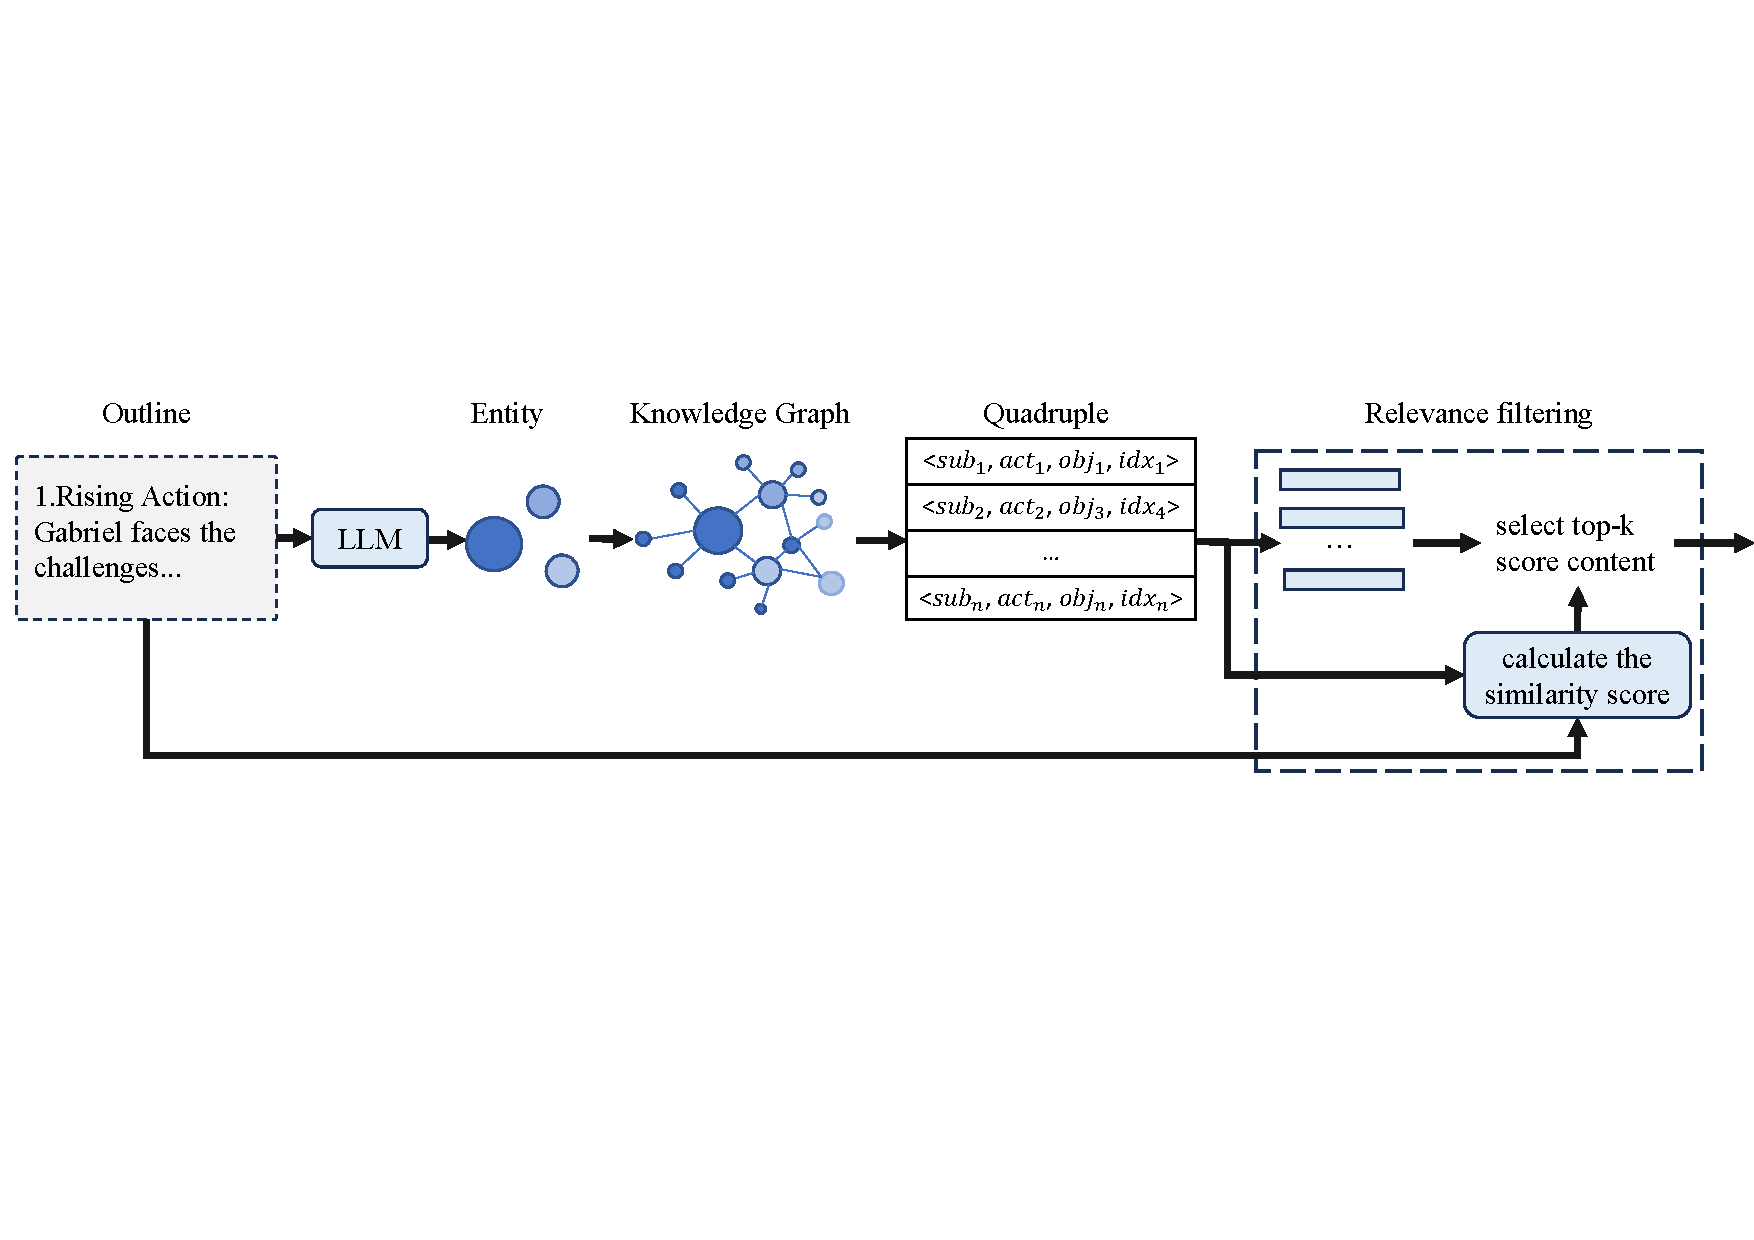
\includegraphics[width=0.96\linewidth]{images/query.pdf}

    \caption{
    The details of querying for the relevant content. Notably the last arrow points to the historical information semantically related to the input content.
    }  
    \label{fig:query}
\vspace{-6pt}
\end{figure*}
\section{Proposed Method}
We propose a dynamic hierarchical outlining with memory-enhancement \hjw{long-form} story generation method, named \textbf{\methodname}, aiming to improve the story coherence from plot and context description. Based on the advanced understanding and generation ability of LLM \cite{liu2023pre}, \methodname~ is mainly composed of two parts: the dynamic hierarchical outline and writing module (\textbf{DHO}) and the KG-based memory-enhancement module (\textbf{MEM}). 
As shown in Fig.~\ref{fig:our_method}, given the user input $I$, including story setting, character introduction, and storyline requirements, the rough outlines of a story are planned at a time under the guidance of the writing theory, ensuring the completeness of the plot. Then, the detailed outline and the corresponding part of the story are generated alternately. It means the detailed outlines are not expanded by the rough outline incrementally until its previous stories are generated, enabling it to adjust to the uncertainty of the previously generated stories, and then the detailed outlines guide the generation of sequential stories. MEM stores user input at the very beginning and the generated story during the writing process. The module provides relevant content in natural language for the generation stage, ensuring contextual consistency. Through the collaboration of these two modules, \methodname~improve the story's coherence from plot and contextual consistency.

\subsection{\hjw{Dynamic Hierarchical Outline Mechanism}}
\label{sec:dho}

\hjw{The hierarchical outline  $H=\{R,D\}$ is composed of a rough outline $R$ and a detailed outline $D$.}\hjw{Previous works have used higher-level attributes like plots or commonsense knowledge to improve the quality of generated stories. We find that certain novel writing theories \cite{TheoryFive, TheorySeven, TheoryTwelve} enhance story generation. By incorporating the novel writing theory \cite{TheoryFive} (see Fig.~\ref{fig:novel}) into the rough outline planning stage, we improve the overall structure. This is done by stating the theory in the rough outline generation prompt. Thus, the rough outline $R$ was generated based on user input $I$:}
\begin{equation}
\label{eq:ROG}
R=LLM(WT,I,P_{rough\_utline}),
\end{equation}

\wqyr{
where $WT$ is the novel writing theory, $LLM(\cdot)$ is LLM inference operation, and $P_{rough\_outlie}$ is the prompt guiding LLM to generate a rough outline.}

The detailed outline \hjw{$D=\{d_i\}_{i=1}^{5}$} is generated step by step according to the corresponding part of the rough outline $r_i$ and its relevant content $RInfo._i$, ensuring its adaptation to the uncertainty in the story generation stage. 
\begin{equation}
\label{eq:DOG}
d_i=LLM(r_i,RInfo._i,P_{detailed\_outline}),
\end{equation}
\wqyr{
where $P_{detailed\_outline}$ is the prompt that indicates LLM to generate a detailed outline. The $d_i=\{do_i^t\}_{t=1}^{M}$ contains detailed outlines expanded from the rough outline. The $M$ is the number of detailed outlines expanded from the given rough outline $r_i$ which should be set at the beginning. 
}

The story content $s_i^t$ is generated step-by-step based on the detailed outline $do_i^t$ and relevant generated content $DInfo._i^t$ of the sub-detailed outline $do_i^t$, \hjw{which is as follows:} 
\begin{equation}
\label{eq:SG}
s_i^t=LLM(do_i^t,DInfo._i^t,P_{gen\_story}),
\end{equation}

\wqyr{where $P_{gen\_story}$ is the prompt that indicates LLM to generate a partial story. The detailed process of writing story $S$ in Algorithm \ref{alg:DO_S}. The details of prompts in the DHO are shown in Appendix~\ref{sup:prompt dho}.
}

\begin{algorithm}[t]
    \caption{Inference Pipeline for \methodname}
    \label{alg:DO_S}
    \begin{algorithmic}[1]
    \small
    \REQUIRE Novel writing theory $WT$, the large language model applied in DOME ${LLM}$, user input $I$, rough outline prompt $P_{rough\_outline}$, detailed outline prompt $P_{detailed\_outline}$, story generation prompt $P_{gen\_story}$.
    \STATE Initialize MEM $KG$.
    \STATE  Generate rough outline $R$ via Eqn. (\ref{eq:ROG}).
        \FOR{$r_i$ in $R=\{r_i\}_{i=1}^{i=5}$}
            \STATE Find relevant content $RInfo_i$ about $r_i$ from $KG$.
            \STATE Generate detailed outlines $d_i$ via Eqn. (\ref{eq:DOG}).
            \STATE Add $d_i$ into $D$.
            \FOR {$do_i^t$ in $d_i=\{do_i^t\}_{t=1}^{t=M}$}
                \STATE Find relevant content $DInfo._i^t$ about $do_i^t$ from $KG$.
                \STATE Generate partial story $s_i^t$ via Eqn. (\ref{eq:SG}).
                \STATE Add $s_i^t$ into story $S$.
                \STATE Store $s_i^t$ into $KG$.
            \ENDFOR
        \ENDFOR
        \RETURN $R$, $D$ and $S$.
    \end{algorithmic}
  
\end{algorithm}

\begin{figure*}[t]
\centering
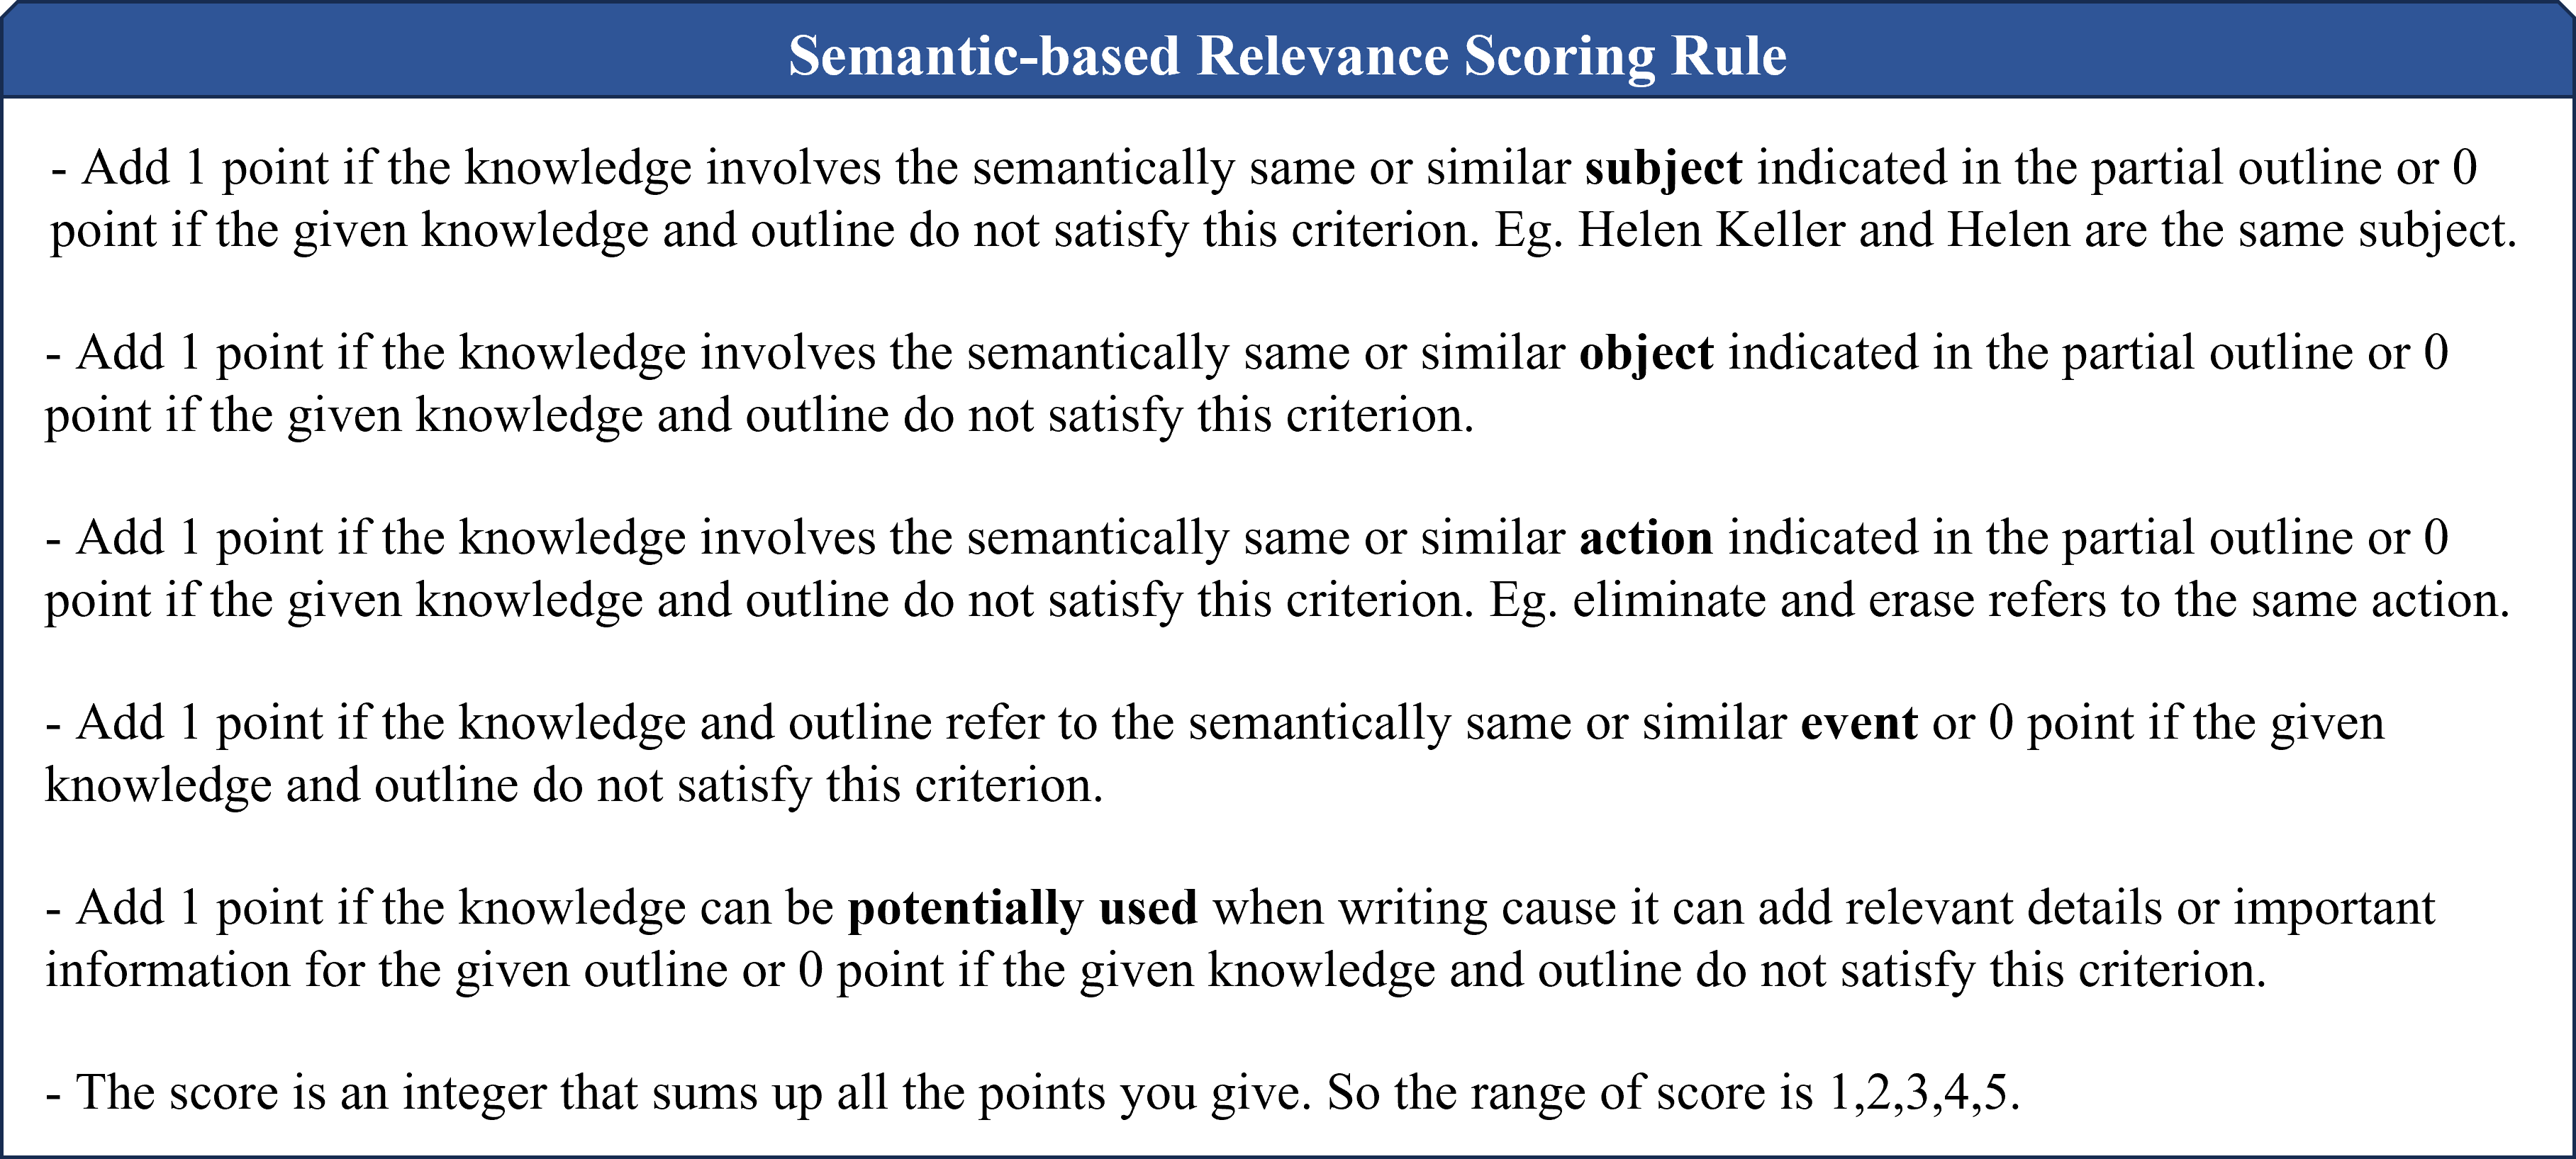
\includegraphics[width=0.92\linewidth]{images/r4.png}

    \caption{
    The criterion of filtering on semantic relevance.
    }  
    \label{fig:critition}
\vspace{-5pt}
\end{figure*}
\subsection{\hjw{Memory-Enhancement Module}}
\hjw{Recently, many works \cite{liu2024lostinmiddle} have} shown that LLMs tend to ignore the information in the middle of the long inputs. As the story generation process progresses, the increasing story length affects the LLM's attention on the relevant content when generating new content, increasing computing overhead \cite{choromanski2020rethinking} and even leading to contextual conflict \cite{Re3}. We propose an additional memory-enhancement module, named \textbf{MEM}, to store the generated story and provide concise relevant content.

KGs and their variants are well-established tools for content storage and query \cite{wen2023mindmap}. KGs extract the key information for the content like subject, action, and object and ignore unimportant information like adverbs and modifiers.
Besides, the structure of the knowledge graph supports reasoning and information fusion, which is conducive to information integration \cite{Pan2023UnifyingLL}.
Based on the analysis above, \hjw{the MEM} applies temporal knowledge graph (TKG) \cite{roddick2002survey} to store the generated story. TKG is stored by quadruples in the form of $<subject, action, object, index>$. The index means the chapter number of the information. The module stores the input story premise at the very beginning and the generated content and provides query-relevant content %(\hjw{see Fig.~\ref{fig: query}}) 
based on entity retrieval in TKG each time the DHO generates content.

\hjw{To store entity, we use LLM to extract triples for every sentence and then add the current chapter number to form quadruples.}
\wqyr{To access the relevant content (see Fig. \ref{fig:query}), we first conduct entity-based quadruple retrieval~\cite{reinanda2020knowledge} on TKG and then apply LLM to filter the retrieved results through semantics correlation by evaluating relevance based on rules (see Fig. \ref{fig:critition}). MEM can provide the $top$-$k$ most relevant information as query-relevant content, making it concise and semantically relevant with input (more details can be seen in Appendix~\ref{sup:mem prompt}).}



\subsection{\hjw{Temporal Conflict Analyzer}}

\wqyr{The evaluation of long-form stories in previous work mainly relies on humans, which is time-consuming and laborious \cite{DOC,improving-pacing}.}
MEM applies TKG to store story and it is easy for TKG to associate context \cite{wen2023mindmap}. Thus we propose an auto metric that measures the contextual consistency of the story by calculating the rate of conflict quadruples to total quadruples. To detect the conflict quadruples, the quadruples in TKG $Q=\{q_{i}\}_{i=1}^{N}$ of generated stories are grouped by rules (\hjw{see Fig.~\ref{fig:grules}  in Appendix \ref{sup:grules}}) sequentially and without repetition and the potential conflict information is aggregated. \wqyr{Since LLm-as-a-judge has been verified by experiments \cite{llm-as-a-judge} and it can evaluate some features of a text within a certain length according to rules \cite{achiam2023gpt, liu-etal-2021-durecdial}, we apply LLM to further detect the conflict quadruples based on time order. More details about the temporal conflict analyzer are reported in Appendix~\ref{sup:mem example}. }In this way, we can find the quadruples $Q^{conflict}=\{q_{i}^{conflict}\}_{i=1}^{m}$ containing conflict information. \hjw{The conflict rate is expressed as follows:}
\begin{equation}
\label{eq:cr.}
CR.=m/N \times 100\%,
\end{equation}
\hjw{where $N$ is the number of quadruples in TKG and $m$ is the number of conflict quadruples in TKG.}
